\documentclass{article}
\usepackage{amsmath}
\usepackage{graphicx}

\begin{document}

\title{Relatório sobre o Dataset Iris}
\author{
  \begin{tabular}{c}
    Enzo Gabriel Silva Miranda \\
    Manuela Silva de Andrade \\
    Isabela Vieira Silva Cruz Martins \\
  \end{tabular}
}

\maketitle

\section{Explicação do Dataset Iris}

O conjunto de dados Iris é um dos conjuntos de dados mais conhecidos e amplamente utilizados na área de aprendizado de máquina. Ele contém informações sobre três espécies diferentes de flores Iris: Setosa, Versicolor e Virginica. Cada espécie é representada por amostras com características morfológicas medidas a partir de suas sépalas (partes externas da flor) e pétalas (partes internas da flor).

\section{Descrição da Base do Dataset}

O dataset Iris é composto por amostras de 150 flores Iris, onde cada amostra possui informações sobre quatro atributos: sepal\_length, sepal\_width, petal\_length e petal\_width. Além disso, cada amostra está associada a uma classe (espécie) específica: setosa, versicolor ou virginica.

\section{Explicação do uso do KNN no código}

O algoritmo K-Nearest Neighbors (KNN) é utilizado no código para realizar a classificação das amostras do dataset Iris. Ele funciona encontrando as \emph{k} amostras mais próximas (vizinhas) a uma amostra de teste com base na distância euclidiana entre seus atributos. A classe mais frequente entre essas \emph{k} amostras é então atribuída à amostra de teste.

\section{Quantidade de Classes, Entropia e Entropia Máxima}

O dataset Iris possui três classes distintas: setosa, versicolor e virginica. Para cada atributo do dataset, calculamos a entropia e a entropia máxima.

\subsection{Entropia}

A entropia é uma medida da incerteza associada à classificação das amostras com base nos valores de um determinado atributo. Pode ser calculada usando a fórmula:

\[
\text{Entropia} = - \sum_{i=1}^{n} p_i \log_2(p_i)
\]

onde $n$ é o número de classes, e $p_i$ é a probabilidade de ocorrência da classe $i$.

\subsection{Entropia Máxima}

A entropia máxima é a entropia ideal quando todas as classes têm a mesma probabilidade. Pode ser calculada usando a fórmula:

\[
\text{Entropia Máxima} = \log_2(n)
\]

onde $n$ é o número de classes.

A seguir estão os valores de entropia e entropia máxima para cada atributo do dataset Iris:

\begin{itemize}
    \item Atributo sepal\_length: Entropia = 1.4950, Entropia Máxima = 1.5849 \\
    (A entropia desse atributo mede a incerteza associada à classificação das amostras com base no comprimento da sépala (parte da flor). A entropia máxima para esse atributo indica que existem diferentes valores de comprimento de sépala presentes no conjunto de dados, o que contribui para a incerteza.)
    
    \item Atributo sepal\_width: Entropia = 1.2594, Entropia Máxima = 1.5849 \\
    (A entropia desse atributo mede a incerteza associada à classificação das amostras com base na largura da sépala. A entropia máxima para esse atributo indica que existem diferentes valores de largura de sépala presentes no conjunto de dados.)
    
    \item Atributo petal\_length: Entropia = 1.5819, Entropia Máxima = 1.5849 \\
    (A entropia desse atributo mede a incerteza associada à classificação das amostras com base no comprimento da pétala (parte da flor). A entropia máxima para esse atributo sugere a presença de diferentes valores de comprimento de pétala no conjunto de dados.)
    
    \item Atributo petal\_width: Entropia = 1.5842, Entropia Máxima = 1.5849 \\
    (A entropia desse atributo mede a incerteza associada à classificação das amostras com base na largura da pétala. A entropia máxima para esse atributo indica a existência de diferentes valores de largura de pétala no conjunto de dados.)
\end{itemize}

\section{Código}

A seguir está o código utilizado para calcular a entropia e entropia máxima:

\begin{verbatim}
import seaborn as sns
import numpy as np
from scipy.stats import entropy
from sklearn.preprocessing import KBinsDiscretizer

# Carregar o conjunto de dados Iris do Seaborn
tips = sns.load_dataset('iris')

# Converter as colunas numéricas em qualitativas usando a discretização
discretizer = KBinsDiscretizer(n_bins=3, encode='ordinal', strategy='uniform')
tips_quantitativos = tips.select_dtypes(include=[np.number])
tips_qualitativos = discretizer.fit_transform(tips_quantitativos)
tips_discretizados = tips.copy()
tips_discretizados[tips_quantitativos.columns] = tips_qualitativos

# Mapear as classes para valores numéricos
class_mapping = {'setosa': 1, 'versicolor': 2, 'virginica': 3}
tips_discretizados['species'] = tips_discretizados['species'].map(class_mapping)

# Calcular a entropia e entropia máxima para cada atributo
for column in tips_discretizados.columns:
    target = tips_discretizados[column]
    classes, counts = np.unique(target, return_counts=True)
    total_count = len(target)
    num_classes = len(classes)
    
    class_probabilities = counts / total_count
    class_entropy = entropy(class_probabilities, base=2)
    max_entropy = np.log2(num_classes)
    
    print(f"Atributo {column}: Entropia = {class_entropy:.4f}, 
    Entropia Máxima = {max_entropy:.4f}")

\end{verbatim}

\begin{figure}[htb]
  \centering
  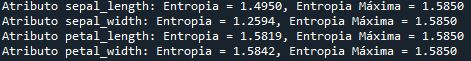
\includegraphics[width=1\linewidth]{Console.JPG}
  \caption{Imagem do Console}
  \label{fig:imagem}
\end{figure}

\section{Conclusão}
Com base na análise da entropia e entropia máxima dos atributos do conjunto de dados Iris, podemos tirar algumas conclusões importantes. A entropia representa a incerteza associada à classificação das amostras em suas respectivas espécies, levando em consideração as características morfológicas medidas.


Observamos que diferentes atributos apresentam níveis variados de entropia. O atributo "sepallength" possui uma entropia relativamente alta, indicando uma distribuição mais equilibrada de valores e maior incerteza na classificação. Por outro lado, os atributos "sepalwidth", "petallength" e "petalwidth" têm entropias mais baixas, sugerindo que eles são mais informativos para distinguir as espécies de flores.

Além disso, a comparação da entropia com a entropia máxima revela que os atributos têm um potencial limitado de informação. A entropia máxima Hmax representa o máximo nível de incerteza possível para a classificação. Se a entropia de um atributo se aproxima da entropia máxima, isso indica que a distribuição dos valores desse atributo é mais equilibrada e, portanto, o atributo é menos discriminativo para a classificação das espécies de flores.


\end{document}
